\section{Project organisatie}

\subsection{Externe Interfaces}
Het project is opgedragen door de VUB in het kader van de lessen ``Software Engineering". De cliënten zijn Ragnhild Van Der Straeten \cite{rvdstrae} en assistent Jens Nicolay \cite{jnicolay}. Later kan deze basis uitgebreid worden naar geleerden binnen en buiten de VUB. 
De communicatie met de cliënten gebeurt langs mail.


\subsection{Interne structuur}
Er zijn verschillende rollen die moeten opgevuld worden.
De rollen en hun functies zijn: 

\begin{itemize}
\item Project Manager
\begin{itemize}
\item Leidt het team
\item Contactpersoon van het team
\item Bemiddelaar tijdens meningsverschillen
\item SPMP
\end{itemize}

\item Configuration Manager
\begin{itemize}
\item Beheert de tools en libraries die gebruikt worden
\item Beheert de GitHub
\item SCMP
\end{itemize}

\item Database Manager
\begin{itemize}
\item Beheert de database
\item SDD
\end{itemize}

\item Design Manager
\begin{itemize}
\item Webdesign
\item Product design
\item SDD
\end{itemize}

\item Test Manager
\begin{itemize}
\item Zorgt dat het programma aan voldoende tests wordt onderworpen
\item STD
\end{itemize}

\item Quality Assurance
 \begin{itemize}
 \item Zorgt voor de kwaliteit van de code
 \item SQAP
 \end{itemize}
 \end{itemize}
 
 \newpage

In de onderstaande tabel staan de functies en de personen die verantwoordelijk en back-up zijn voor deze functies.

\begin{table}[h]
\centering
\begin{tabular}{c|c|c}
\textbf{Rol} & \textbf{Verantwoordelijke} & \textbf{Back-up}  \\
\hline
 Project Manager & Wout Van Riel & Mathieu Reymond \\
 Test Manager & Yannick Verschueren & Arno Moonens \\
 Design & Mathieu Reymond & Yannick Verschueren \\
 Quality Assurance & Yannick Verschueren & Arno Moonens \\
 Database Manager & Arno Moonens & Sam Vervaeck \\
 Config Manager & Sam Vervaeck & Wout Van Riel 
\end{tabular}
\caption{Rolverdeling}
\label{tab:rolverdeling}
\end{table}

Er wordt gecommuniceerd in de groep met behulp van slack \cite{Slack} en mail. 

\subsection{Werkplanning}
In volgende Gant-chart is de werkplanning tot de volgende deadline te zien.
\newline

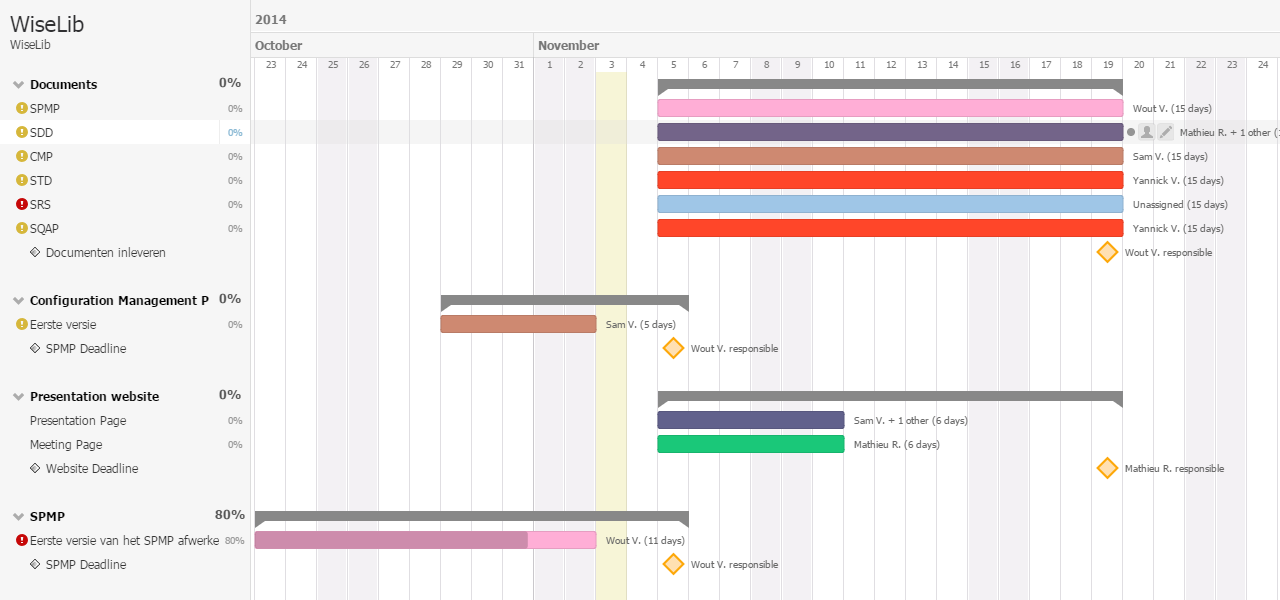
\includegraphics[width=\linewidth]{Gant_chart}
